%% ID: falling_balls
%% TITLE: Falling Balls
%% TYPE: question
%% QUESTIONTYPE: symbolic
%% CONCEPTS: energy, momentum, momentumii, eq_of_motion_diff
%% VIDEOS: 
%% LEVEL: 4
%% TOPIC: mechanics/dynamics
%% ORDER: 9

\begin{problem}[HSC1946P1X1a] % reference to coefficient of restitution removed
{%\begin{enumerate}
%  \item State Newton's laws of motion and show how they lead to the statement that the force acting on a body is equal to the rate of change of momentum of that body if the units are suitably chosen.
%  \item 
Steel balls of mass \valuedef{m}{0.1}{kg} are dropped from a height of \valuedef{h}{5}{m} onto a smooth steel plate inclined at \valuedef{\theta}{45^{\circ}}{}  to the vertical.  If the balls are dropped at the rate of \valuedef{n}{100}{s\sup{-1}}, what is the average force on the plate? You may assume that the collisions between the ball and the plate are elastic and that each ball hits the plate only once.
% \end{enumerate}
}{\stress{Adapted with permission from UCLES, Higher School Certificate Physics, June~1946, Paper~1.}
}{ %Question number missing - X
A diagram is, as always, the first step. They key quantities to show are the height, the speed just before impact, the speed just after impact and the angles involved; as in Figure \ref{fig:Dynamics_ball_plane_p}.

\begin{figure}[h]
	\centering
	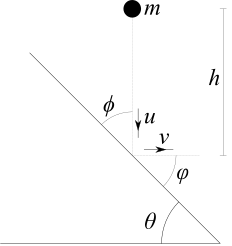
\includegraphics[width=0.3\textwidth]{../../../figures/Dynamics_ball_plane_p.svg}
	\caption{}
	\label{fig:Dynamics_ball_plane_p}
\end{figure}

The force on the plane will be given by Newton's Second Law, \valuedef{\vtr{F}}{\frac{\d\vtr{p}}{\d t}}{}, and so we need to find the momentum change of the steel balls when they bounce off the plate. When a ball collides with the plate, the plate exerts an impulse on the ball to change its momentum; but this impulse has to be perpendicular to the surface, so we can conserve momentum parallel to the plane and conserve energy since the collision is elastic.

The speed, \vari{u}, of the ball as it hits the plate can be found by conserving energy as its gravitational potential energy becomes kinetic energy:
\begin{eqnarray*} 
mgh &= \frac{1}{2}mu^{2} \\ 
u &= \sqrt{2gh}
\end{eqnarray*}

Returning to the collision with the plate, conservation of momentum parallel to the plate gives:
\begin{eqnarray*}
 mu\cos(\phi) &= mv\cos(\varphi) \notag \\ 
 v\cos(\phi) &= u\cos(\varphi) \label{ball_plate_CoM} 
 \end{eqnarray*}
and conservation of energy gives:
\begin{eqnarray*}
 \frac{1}{2}mu^{2} &= \frac{1}{2}{m}v^{2} \notag \\ 
 u^{2} &= v^{2} \notag \\ 
 u &= v \label{ball_plate_CoE} 
\end{eqnarray*}
and then using the result from Equation \eqref{ball_plate_CoE} in Equation \eqref{ball_plate_CoM} gives:
\begin{eqnarray*} 
v\cos(\phi) &= u\cos(\varphi) \\ 
\cos(\phi) &= \cos(\varphi) \\ 
\phi &= \varphi
\end{eqnarray*}
Strictly, \valuedef{\phi}{\varphi}{} plus any multiple of \quantity{2\pi}{}, but that gives the same result.

To find the momentum change which produces the force on the plane; look at the momentum perpendicular to the plate:
\begin{eqnarray*}
 \Delta p &= \text{Final Momentum} - \text{Initial Momentum} \\ 
 &= (-mv\cos(\phi)) - (mv\cos(\phi)) \\ 
 &= -2mv\cos(\phi) 
 \end{eqnarray*}
where the minus sign comes from the fact we have chosen the direction out of the plate as positive. Newton's Second Law then gives:
\begin{eqnarray*} 
F &= \frac{\d p}{\d t} \\ 
&= \frac{N \Delta p}{\Delta t} \\ 
&= n\Delta p \\ &= -2nmv\cos(\phi) \\ 
&= -2\sqrt{2gh}\;nm\cos(\phi) 
\end{eqnarray*}
where N is the total number of balls dropped in a time \vari{\Delta t} and again the minus sign shows that the force is directed into the plate, as expected.

So the force the balls exert on the plate is \valuedef{-2\sqrt{2gh}\;nm\cos(\phi)}{2\sqrt{gh}\;nm}{}. Using the rest of the numbers from the question gives:
\begin{equation*} 
\text{Force} = 2\sqrt{(9.8)(5)}(100)(0.1)= \mbox{\quantity{140}{N}} 
\end{equation*}
}
\end{problem}